\section{Benchmark NIST-10 "Interior Line Singularity"}
\label{sec:bench-10}

This is another example with anisotropic solution that is suitable for testing
anisotropic element refinements. The equation solved is the Poisson's equation.

\begin{equation} \label{interior}
-\Delta u = f
\end{equation}
in the domain $\Omega = (-1, 1)^2$, equipped with a zero
Neumann boundary condition on left edge, Dirichlet boundary
conditions given by the exact solution on the rest of the boundary.
The exact solution is
$u(x,y) = \cos(Ky)\ (x \le 0)$ and $u(x,y) = \cos(Ky) + x^{\alpha}\ (x > 0)$,
where $K$ and $\alpha$ are constants.
The right-hand side $f$ is calculated by inserting exact solution into (\ref{interior}).
The solution of NIST-10 containing a line singularity with $K = \pi/2$ and
$\alpha = 2.01$ is shown in Fig. \ref{fig:sln-nist10}.

\begin{figure}[!ht]
\centering
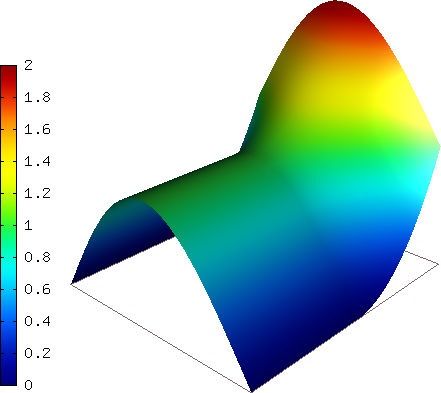
\includegraphics[height=5cm]{nist/nist-10/solution.png}
\caption{The solution to NIST-10 benchmark problem.}
\label{fig:sln-nist10}
\end{figure}

\begin{figure}[!ht]
\centering

\includegraphics[height=5cm]{nist/nist-10/mesh_hp_aniso_init.png}\ \
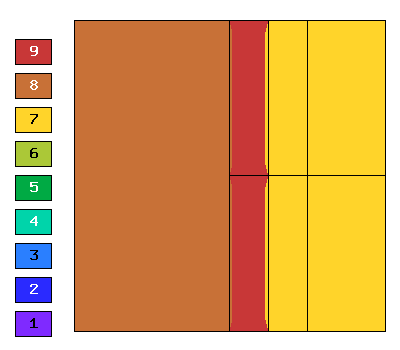
\includegraphics[height=5cm]{nist/nist-10/mesh_hp_aniso.png}
\caption{Initial mesh (left) and final mesh (right) with 381 DOF and the resulting relative error estimate in $H^1$-norm of 8.68994e-05 \% for $hp$-FEM with anisotropic refinements.}
\label{fig:nist-10-hp-aniso}
\end{figure}

\begin{figure}[!ht]
\centering
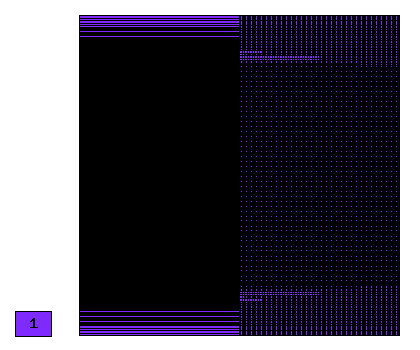
\includegraphics[height=5cm]{nist/nist-10/mesh_h1_aniso.png}\ \
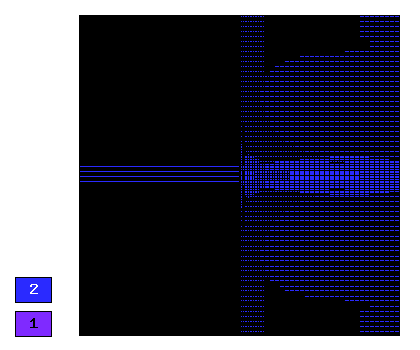
\includegraphics[height=5cm]{nist/nist-10/mesh_h2_aniso.png}
\caption{Final mesh for $h$-FEM with linear and quadratic elements.}
\label{fig:nist-10-h-aniso}
\end{figure}

Figs. \ref{fig:nist-10-conv} compare all
three approaches to automatic adaptivity from the point
of view of DOF and CPU convergence.

\begin{figure}[!ht]
\centering
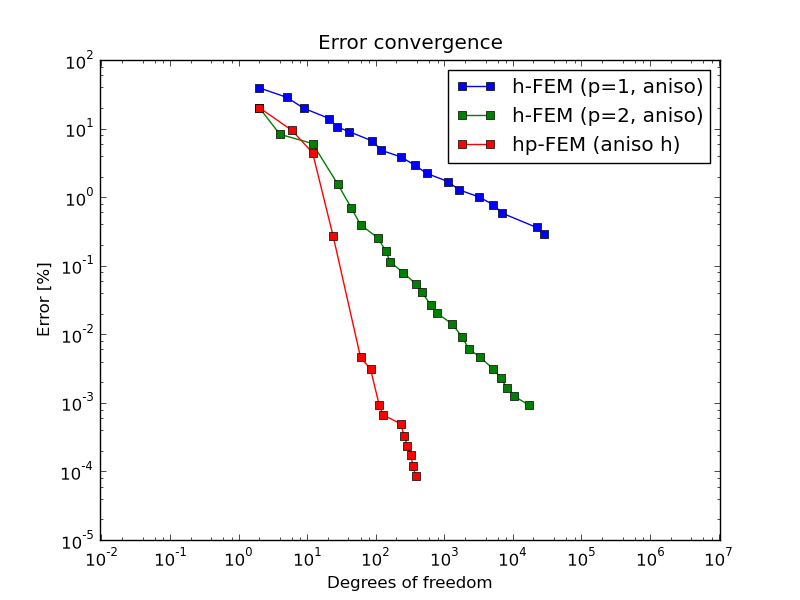
\includegraphics[height=5cm]{nist/nist-10/conv_dof_aniso.png}\ \
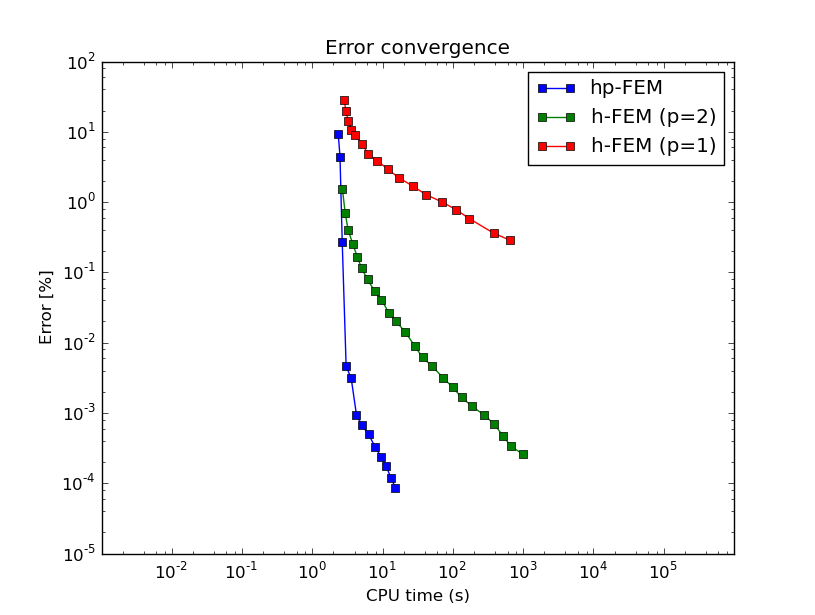
\includegraphics[height=5cm]{nist/nist-10/conv_cpu_aniso.png}
\caption{DOF and CPU time convergence graphs.}
\label{fig:nist-10-conv}
\end{figure}

